\chapter{Analysis and Results}
\label{cap:AnalysisandResults}

This chapter presents the analysis and results of standby traffic and event captures. First the standby traffic is analysed to identify traffic irrelevant to the event objectives triggered. This is followed by a section for each event including analysis and results of overall event characteristics, protocol detection and packet sequences resulting in a signature detection algorithm. \gls{WAN} traffic is compared with the corresponding \gls{WLAN} traffic to identify if these signatures are applicable in both transmissions domains. 

\section{Standby Traffic}
This section presents the analysis of the captured \textit{Standby traffic} to identify traffic patterns or protocols to exclude in further event analysis. First an analysis of the relevance of the different identified protocols is conducted. All occurring traffic patterns within the standby event can be found in the event captures as well, but are irrelevant for the actual event triggering.

The standby event capturing was conducted from 8th of January to 22th of January 2023 in \textbf{Oslo} environment. During this time period there was no physical or application interacting with the Irobot Roomba, all traffic captured was therefore generated by the Irobot Roomba or the connected Irobot cloud service. This traffic is not created by any human interaction and not exposing any private information. Beforehand, the Irobot Roomba had been installed and operated for one month, ensuring that it was in an operating and not installation state. Smart home map, room dividers and customized cleaning jobs were configured. 

Wireshark protocol hierarchy analysis tool was used to display protocol statistics and Table \ref{tab:ProtocolStatistics} presents the protocols and distribution of them. Approximately 50\% of the captured traffic was identified as \gls{UDP} traffic, this is mainly \gls{DNS} but also some NTP and \gls{DHCP} traffic. Another 26.2\% was \gls{TCP} where the majority of the captured traffic is \gls{TLS} which is used by the Irobot Roomba to ensure end-to-end encryption with the cloud server. The last protocol identified was \gls{ARP} representing 24,6\% of the standby traffic. 


\begin{table}[H]
\centering
\caption{Protocol hierarchy and statistics in standby traffic capture }
\label{tab:ProtocolStatistics}
\begin{tabular}{|c|c|c|c|}
\hline
\multicolumn{1}{|c|}{\textbf{Transport protocol}} & \textbf{Percentage}     & \textbf{Service protocol} & \textbf{Percentage} \\ \hline
\multirow{3}*{UDP}                              & \multirow{3}*{49,2} & \gls{DHCP}    & 0,1            \\ \cline{3-4} 
                                                  &                         & \gls{DNS}                       & 48,6                \\ \cline{3-4} 
                                                  &                         & NTP                       & 0,4                 \\ \hline
TCP                                               & 26,2                    & NA                        & NA                  \\ \hline
ARP                                               & 24,6                    & NA                        & NA                  \\ \hline
\end{tabular}
\end{table}

The network architecture in \textbf{Oslo} and \textbf{Drammen} creates a single broadcast domain between the AP, capturing platform and the \gls{ISP} router. As devices only use physical layer \gls{MAC} addresses to communicate on the \gls{LAN} they need \gls{ARP} to create an \gls{IP} to \gls{MAC} forwarding table. \gls{ARP} traffic is therefore broadcasted between these devices requesting updates on \gls{IP} to \gls{MAC} information. The captured \gls{ARP} traffic is not generated by the vacuum cleaner in another broadcast domain and is added as a part of the basefilter with the logical expression \textit{!arp}.

The \gls{ISP} modem is by default configured as the local \gls{DHCP} server allocating, reserving and leasing \gls{IP} addresses to devices connected to the \gls{LAN}. To ease the detection of the simulated \gls{WAN} traffic a \gls{DHCP} reservation was configured on the \gls{ISP} routers for the AP's \gls{LAN} \gls{MAC} address in both \textbf{Oslo} and \textbf{Drammen}. This kept the simulated \gls{WAN} address from changing during capturing and potentially lose traffic. \gls{DHCP} traffic was still needed to be exchanged between the \gls{AP} and the \gls{ISP} modems requesting and verifying that the reserved \gls{DHCP} leases still were active during capturing. \gls{DHCP} traffic in the \gls{LAN} capture is therefore only generated by the \gls{AP} and the \gls{ISP} modem and was added to the basefilter with the logical expression \textit{!dhcp}.

The most dominant protocol in the standby capture was \gls{DNS} with 49.2\% of the packets. 98.3\% of these \gls{DNS} packets were requests and responses for the \gls{DNS} A record for \gls{FQDN} \textit{a.root-servers.net}, this traffic flow is shown through Wireshark in Figure \ref{fig:dns_a-root}. This is one of the \gls{DNS} top level domain servers in the \gls{DNS} hierarchy and will only point to top level domain server such as .com, .org and .no. By analyzing the management console of the AP, it was observed that the \gls{AP} requested the \gls{DNS} record for \textit{a.root-servers.net} to determine if it had Internet connectivity or not. A successful response will indicate Internet connectivity. These \gls{DNS} packets are therefore irrelevant in the analysis of Irobot Roomba traffic and are specifically excluded in a Wireshark filter for further \gls{DNS} analysis with the following filter  \textit{((dns) \&\& !(frame.len ==78 or frame.len ==94))}. Frame lengths of 78 and 94 bytes are used to identify the \gls{DNS} request and response in Figure  \ref{fig:dns_a-root}

\begin{figure}[H]
    \centering
    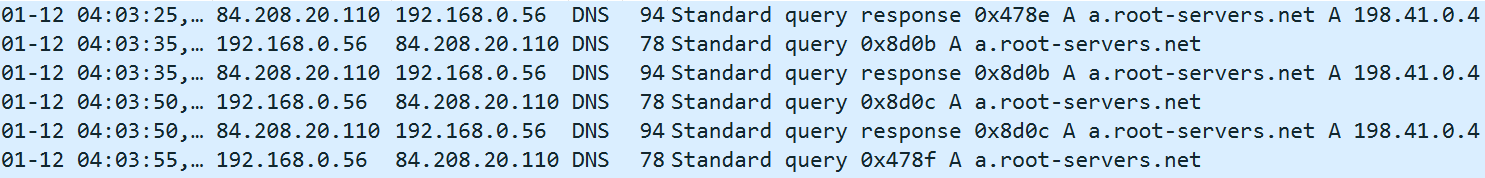
\includegraphics[width=\textwidth]{figures/DNS_a-root.png}
    \caption{Reoccurring DNS traffic associated with a.root-server.net}
    \label{fig:dns_a-root}
\end{figure}

When the filter was applied only 174 \gls{DNS} packets were left. In the remaining \gls{DNS} traffic it was observed several \gls{DNS} requests and responses generated by the \gls{AP} towards the TP-Link cloud services, these \gls{FQDN}s are listed below and shown in Figure \ref{fig:tp-link_fqdn}. 

\begin{itemize}
    \item n-devs-gw.tplinkcloud.com
    \item n-deventry-gw.tplinkcloud.com
\end{itemize}

\begin{figure}[H]
    \centering
    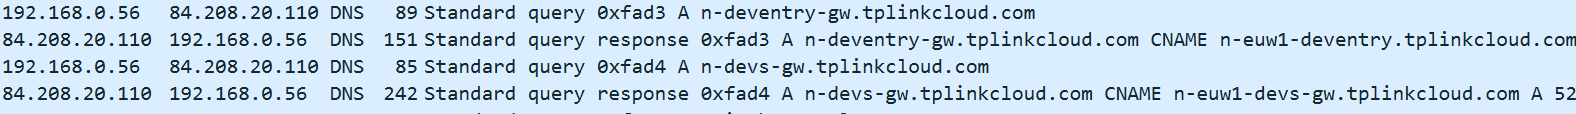
\includegraphics[width=\textwidth]{figures/DNS-tp-link.png}
    \caption{DNS traffic generated by the \gls{AP} towards TP-Link cloud services}
    \label{fig:tp-link_fqdn}
\end{figure}

These \gls{DNS} packets are excluded because they are related to the \gls{AP} and not the \gls{RVC}. After exclusion only four different \gls{FQDN} requests generated by the Irobot Roomba were displayed. Three of the \gls{FQDN} are towards the \textit{.irobot} domain and the last one is a part of .\textit{amazoneaws}. Amazone \gls{AWS} is a large provider of cloud services and bought Irobot cooperation in 2022 \cite{irobot2023_amazone} and is therefore using Amazone \gls{AWS} for their cloud services. These \gls{FQDN}s are listed below. 

\begin{itemize}
    \item 0.irobot.pool.ntp.org
    \item disc-prod.iot.irobotapi.com
    \item unauth1.prod.iot.irobotapi.com
    \item a2uowfjvhio0fa.iot.us-east-1.amazonaws.com
\end{itemize}

All \gls{DNS} traffic generated by the Irobot Roomba are occurring regularly throughout the entire standby traffic time period, this is presented in Figure \ref{fig:dns_irobot_graph}. Irobot's public NTP server \textit{0.irobot.pool.ntp.org} is requested each 12th hour,  in the project's standby traffic this is at 03:36 and 15:36. This is used to synchronize the local clock on the Irobot Roomba to a global time zone, allowing all actions or smart features using time to operate correct. \textit{disc-prod.iot.irobotapi.com}, \textit{unauth1.prod.iot.irobotapi.com} and \textit{a2uowfjvhio0fa.iot.us-east-1.amazonaws.com} are all requested once a day at the same time. The function of these requests are not identified, but when trying to access the \gls{FQDN}s through Google Chrome it prompts \textit{"Missing Authentication Token"}, based on the naming convention of the \gls{FQDN}s it is easy to believe that they are used for re-authentication of the Irobot Roomba. 

\begin{figure}[H]
    \centering
    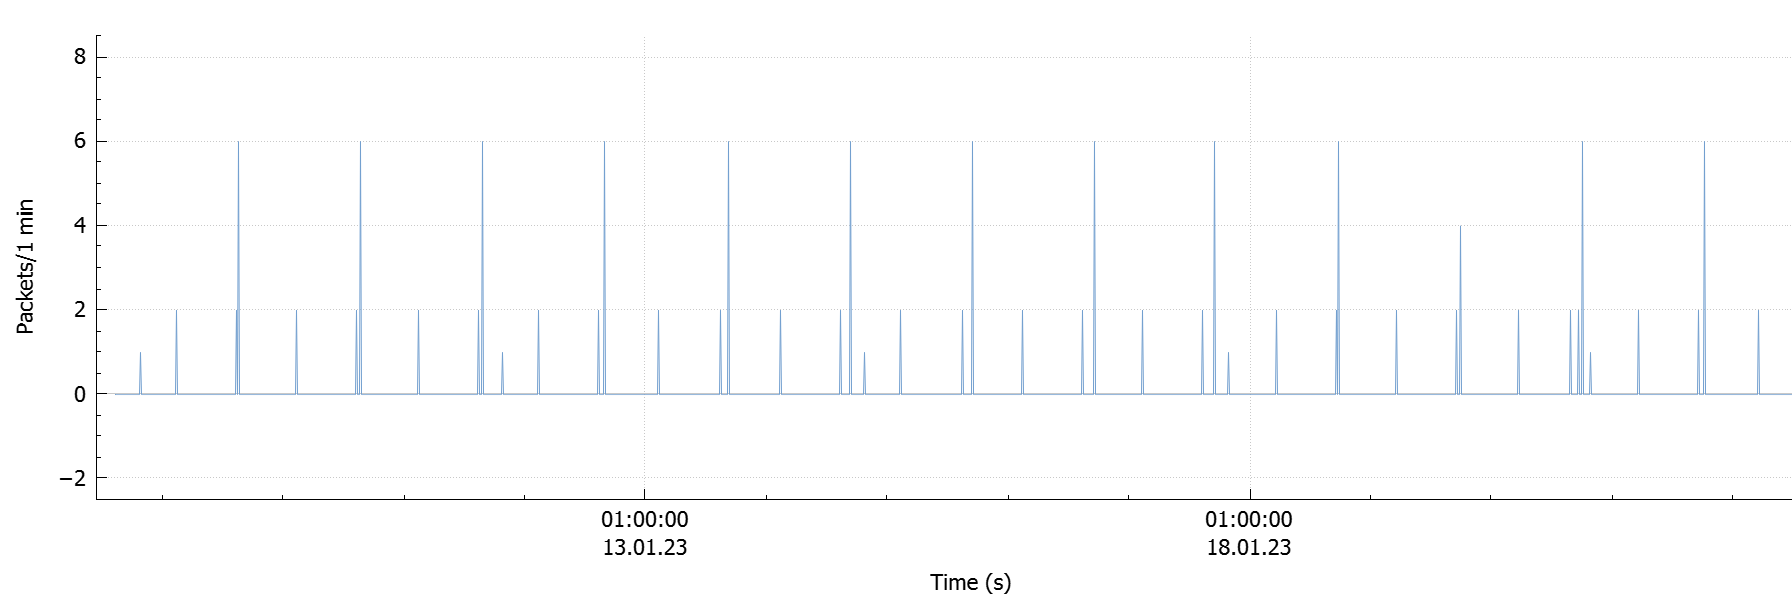
\includegraphics[width=\textwidth]{figures/DNS_irobot_graph.png}
    \caption{Irobot's reoccurring \gls{DNS} traffic presented in graphical view}
    \label{fig:dns_irobot_graph}
\end{figure}

The \gls{DNS} observations identifies that the Irobot Roomba is depending on \gls{DNS} to be able to access Irobot's cloud services. This protocol is a potential indication of cloud functionality, used or access by the Irobot Roomba and is included in further analysis of events. \gls{DNS} request for \textit{a.root-servers.net} had to be excluded due to the large amount. All Irobot generated \gls{DNS} requests had a packet size larger then 78 bytes as shown in Figure \ref{fig:dns_a-root} and all responses were larger then the response for \textit{a.root-server.net}. As the \gls{DNS} response is the most interesting part of the communication it is safe to exclude all \gls{DNS} packets smaller then 94 bytes without missing any \gls{DNS} responses towards the Irobot domains. 

\gls{NTP} server-client sessions are identified every 30 minutes generating a large volume of \gls{NTP} traffic. When observing \gls{DNS} requests to Irobot's public \gls{NTP} service \textit{0.irobot.pool.ntp.org} and \gls{NTP} traffic in Wireshark it is possible to identify that the Irobot Roomba is changing the corresponding \gls{NTP} server every time the \gls{DNS} response is received, this is shown in Figure \ref{fig:irobot_ntp_dns}. Since the \gls{NTP} traffic is continuous it is not related to events triggered, and can be excluded from further analysis by adding the logical expression \textit{!ntp} to the basefilter.

\begin{figure}[H]
    \centering
    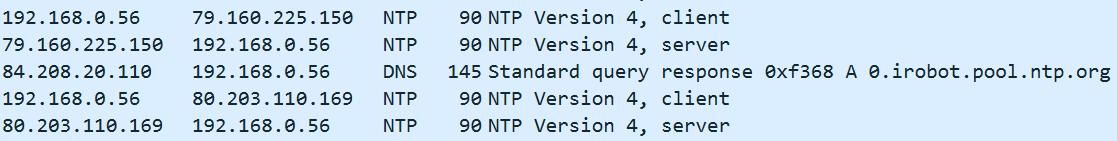
\includegraphics[width=\textwidth]{figures/NTP-irobot.png}
    \caption{Irobot NTP client-server traffic}
    \label{fig:irobot_ntp_dns}
\end{figure}

\gls{TCP} traffic was analyzed in the same manner as the network service protocols \gls{ARP}, DHCP, \gls{DNS} and \gls{NTP}. Remaining \gls{TCP} traffic is then displayed in Wireshark and is shown in Figure \ref{fig:tcp_keep-alive}. Wireshark's protocol hierarchy statistic tools identified that 64.4\% of the remaining \gls{TCP} packets uses \gls{TLS} to secure the connection, this aligns with the observations in Figure \ref{fig:tcp_keep-alive} where the reoccurring \gls{TCP} pattern consists of two \gls{TLS} packets including payload information and one empty \gls{TCP} acknowledge packet confirming that the last packet was received. Continuous \gls{TCP} traffic is generated to keep the \gls{TCP} connection between the Irobot Roomba and the cloud service open as \gls{TCP} has a timeout value on all session. The majority of smart environments are installed behind \gls{NAT} and the \gls{TCP} session must therefore be initiated from the distributed \gls{IoT} devices.  Keep-alive traffic includes the least amount of data needed to keep the connection alive or continuously updated. All event specific packets are therefore larger than 97 bytes.  This filter is combined with the \gls{DNS} packet length filter and is applied with the logical expression \textit{(frame.len > 97)} excluding all packets less than 97 bytes.

\begin{figure}[H]
    \centering
    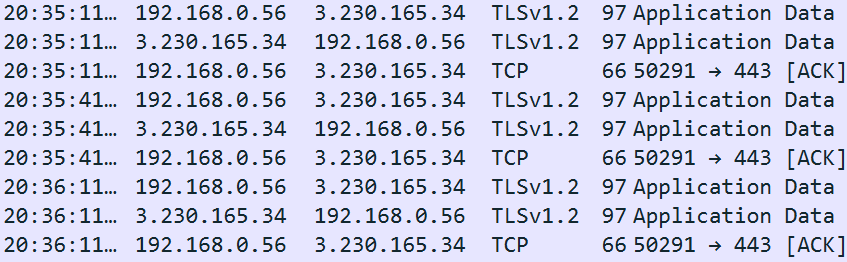
\includegraphics[width=\textwidth]{figures/tcp_keep-alive.png}
    \caption{Roccuring \gls{TCP} traffic from the standby capturing displayed in Wireshark}
    \label{fig:tcp_keep-alive}
\end{figure}

Commando and control traffic from the Irobot's cloud services is generated from the same corresponding host as the TCP-keep-alive traffic. To identify the \gls{FQDN} used in this session establishment, a combined filter with \gls{DNS} and \gls{TCP} is applied, as shown Figure \ref{fig:tcp_keep-change_dns}. As presented the Irobot Roomba terminated the \gls{TCP}-keep-alive session right before a \gls{DNS} request is sent for \textit{a2uowfjvhio0fa.iot.us-east-1.amazonaws.com}, and a new session is established with one of the \gls{IP} addresses in the \gls{DNS} response. After the establishment of the new session there is uploaded data to the new host, probably synchronising and updating current status on the Irobot Roomba.

An attacker will have to eavesdrop traffic for less than 24 hours to be able to identify which \gls{TCP} session belongs to the Irobot Roomba. In a large scale eavesdropping attack attackers can trigger actions based on identification of this \gls{DNS} response, knowing that a Irobot vacuum cleaner is establishing a new session with one of the responded \gls{IP} addresses. 


\begin{figure}[H]
    \centering
    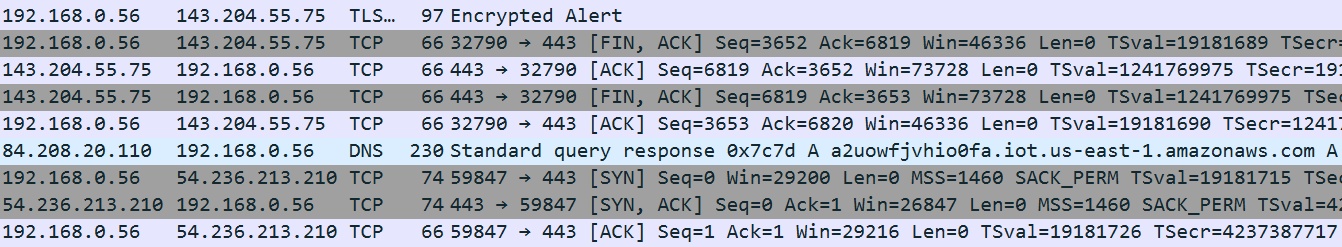
\includegraphics[width=\textwidth]{figures/wireshark_irobot_cloud_dns.png}
    \caption{Identification of Irobot commando and control traffic displayed in Wireshark}
    \label{fig:tcp_keep-change_dns}
\end{figure}

A base filter is created based on the observations described earlier in this section to exclude irrelevant standby traffic from further analysis of events. \gls{DNS} online verification generated by the \gls{AP} and \gls{TCP}-keep-alive traffic is excluded with the same logical expression excluding all packets smaller then 98 bytes, \textit{(frame.len > 97)}. This leaves the \gls{DNS} responses to other Irobot cloud services which can be used for service attribution. \gls{ARP}, \gls{DHCP} and \gls{NTP} are excluded due to functionality. The base filter created and used in following analysis of event captures are presented below. When this filter was applied to the \textit{Standby traffic} capture the total number of packets was reduced from 5,052,284 to 4,010 displaying only 0.8\% of the captured traffic.

\begin{itemize}
    \item \textit{(!ntp \&\& !dhcp \&\& !arp \&\& frame.len > 97)}
\end{itemize}


\section{General Event Analysis}

 This section introduces the general capturing process conducted in both \textbf{Oslo} and \textbf{Drammen} environment. Considerations and observations used during the event triggering process are also presented. 

 Capturing is started on the Raspberry PI for both \gls{WLAN} and \gls{LAN}, filters used on \gls{WLAN} captures are the same in both environments due to static \gls{WLAN} \gls{MAC} address for the Irobot Roomba. This \gls{MAC} address is found through the Irobot home application. However the simulated \gls{WAN} address is different, in Oslo environment is was 192.168.0.56 and in Drammen is was 192.168.0.91, the reason for this was that the \gls{IP} address reserved in Oslo was already in use within the Drammen \gls{LAN}. Tshark commands for \gls{WLAN}, Oslo \gls{LAN} and Drammen \gls{LAN} is listed below. 

 \begin{itemize}
     \item \gls{WLAN}: \textit{sudo tshark -i wlan1 -f 'eth.host 50:6F:0C:2F:EB:A2' -w 'output.pcap'}
     \item Oslo: \textit{sudo tshark -i eth0 -f 'ip.host "192.168.0.51' -w 'output.pcap'}
     \item Drammen: \textit{sudo tshark -i eth0 -f 'ip.host "192.168.0.91' -w 'output.pcap'}
 \end{itemize}

 The initiated capture was continuous running in both environments during the entire event triggering, since the output files never exceeded 500MB. During the capturing all event objectives were triggered 10 times per environment, resulting in 20 captures per event in total. All cleaning events were triggered and identified as finished when the smart home application prompted a "finished cleaning" notification. Both start and end time for all events was noted and used in the event file extraction. 

 When all event triggering was conducted, the capturing was stopped and the environment capturing file, including all triggered events, were extracted to another computer via WinSCP file transfer application. The pcap files were opened in Wireshark and a time filter was applied to extract individual files for each of the different triggered events, resulting in 20 different files for each of the event objectives. Timefilter syntax and example is presented below. 
 \begin{itemize}
     \item \textit{(frame.time >= "Month day, year hh:mm:ss") \&\& (frame.time <= "Month day, year hh:mm:ss") }
     \item \textit(frame.time >= "Jan 1, 2023 01:00:00") \&\& (frame.time <= "Jan 2, 2023 20:59:59") 
 \end{itemize}

 The basefilter is applied to all event files excluding the irrelevant traffic identified in \textit{Standby traffic} analysis, traffic left is then associated to actions or events triggered on the vacuum cleaner. Wireshark's protocol hierarchy tool was used to identify the protocol distribution of the events, further calculations about packets and bytes sent during the events were performed with a python scripts. Packet length sequences were extracted with python and manual analysis is used to identify common traffic patterns within each event. All observed patterns or characteristic were compared and used to create a event signature and detection algorithm. 

 These detection algorithms are applied to all 120 event files to evaluate the level of detection and to compare the different signatures with each other. If an algorithm have more then 90\% detection rate and not identified in any other event objectives, it was possible to attribute.

 \section{Automated Cleaning}

This section introduce specific configuration and decisions during \textit{Automated cleaning} event and analysis. The results from the analysis will be presented at the end of the section. 
 
\textit{Automated cleaning} is integrated with IFTTT location service and a cleaning event is triggered when the user's phone is observed more than 200 meters away from the smart environment postal address. Start time is noted when a notification is received and event end is noted when a notification for finished cleaning is received. Due to time constrains during this master project several \textit{Automated cleaning} events were triggered on the same day. Irobot restrictions only allow one triggering of these events each day, so the executed customized cleaning was deleted and then reconfigured after event end. This allowed more then one event per day.

Triggering date and time for all \textit{Automated cleaning} events are presented for \textbf{Oslo} in Table \ref{tab:AC_dateandtimeOslo} and \textbf{Drammen} in Table \ref{tab:AC_dateandtimeDrammen}. The triggering of these events in \textbf{Drammen} follows a unrealistic time schedule due to limited availability of the smart environment. However the triggering in \textbf{Oslo} environment was triggered without recreating the cleaning configuration, executing one event per day. Attribution of this event exposes detailed information about the user's routines, and when the environment was empty. 

\begin{table}[H]
\centering
\caption{Automated cleaning triggering date and time overview for Oslo}
\label{tab:AC_dateandtimeOslo}
\begin{tabular}{|c|c|c|c|}
\hline
\textbf{Event} & \textbf{Date} & \textbf{Start time} & \textbf{End time} \\ \hline
1              & 21.02.2023         & 21:06               & 21:14             \\ \hline
2              & 22.02.2023         & 07:37               & 07:45             \\ \hline
3              & 23.02.2023         & 10:10               & 10:16             \\ \hline
4              & 01.03.2023         & 07:42               & 07:47             \\ \hline
5              & 02.03.2023         & 11:05               & 11:10             \\ \hline
6              & 03.03.2023         & 07:03               & 07:08             \\ \hline
7              & 06.03.2023         & 07:04               & 07:09             \\ \hline
8              & 07.03.2023         & 08:42               & 08:47             \\ \hline
9              & 08.03.2023         & 07:49               & 07:54             \\ \hline
10             & 09.03.2023         & 07:22               & 07:29             \\ \hline
\end{tabular}
\end{table}

 \begin{table}[H]
\centering
\caption{Automated cleaning triggering date and time overview for Drammen}
\label{tab:AC_dateandtimeDrammen}
\begin{tabular}{|c|c|c|c|}
\hline
\textbf{Event} & \textbf{Date} & \textbf{Start time} & \textbf{End time} \\ \hline
1              & 25.02.2023         & 21:32               & 21:50             \\ \hline
2              & 26.02.2023         & 01:53               & 02:10             \\ \hline
3              & 26.02.2023         & 15:43               & 15:55             \\ \hline
4              & 26.02.2023         & 17:00               & 17:12             \\ \hline
5              & 26.02.2023         & 22:11               & 22:23             \\ \hline
6              & 27.02.2023         & 07:57               & 08:10             \\ \hline
7              & 27.02.2023         & 08:51               & 09:02             \\ \hline
8              & 27.02.2023         & 11:03               & 11:13             \\ \hline
9              & 27.02.2023         & 12:04               & 12:16             \\ \hline
10             & 27.02.2023         & 13:36               & 13:48             \\ \hline
\end{tabular}
\end{table}

Protocol distribution shows that there are two \gls{DNS} response packets in each of the event files, the rest of the traffic is \gls{TCP} where the majority are \gls{TLS} encrypted. \gls{TCP} packets without \gls{TLS} is either \gls{TCP} acknowledgement packets without payload or a part of a \gls{TCP} three-way-handshake or tare-down. When the event is triggered it is observed an increase in packets between the Irobot Roomba and the corresponding Irobot cloud server, this communication is at a consistent level until a cleaning is done. Then a \gls{DNS} response for \gls{FQDN} \textit{0550315.ingest.sentry.io} is received and a new \gls{TCP} session to one of the responded \gls{IP} addresses is established. The entire corresponding \gls{TCP} session from Oslo environment event 5 is shown in Figure \ref{fig:AC_DNS_ingest}, this is consistent for all \textit{Automated cleaning} events. After this session is finished, a new \gls{DNS} response for \gls{FQDN} \textit{s3.amazoneaws.com} is received and a new \gls{TCP} session is established to one of the responded \gls{IP} addresses.  

\begin{figure}[H]
    \centering
    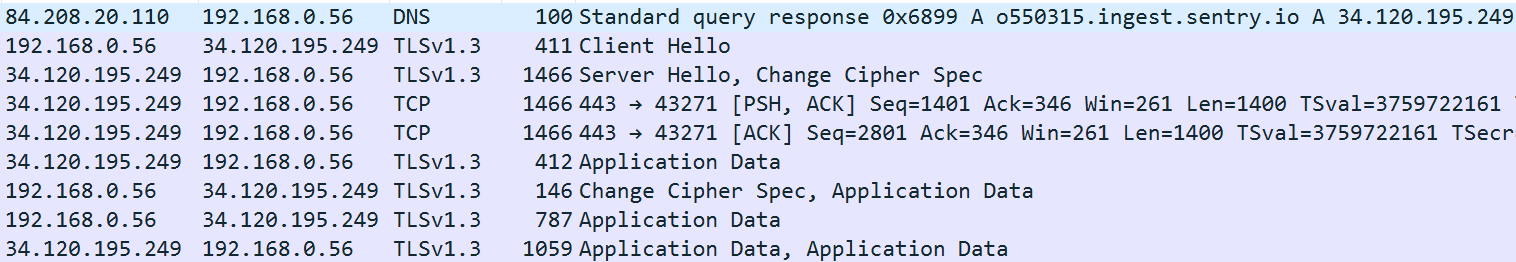
\includegraphics[width=\textwidth]{figures/irobot_AC_DNSimgset.png}
    \caption{TCP session between Irobot Roomba and \textit{0550315.ingest.sentry.io}, initiated after a cleaning is finished}
    \label{fig:AC_DNS_ingest}
\end{figure}


Calculations of number of bytes and  number of packets with associated average and \gls{SD} are presented in Table \ref{tab:ACoverallOSL} and Table \ref{tab:ACoverallDRA}. As presented, the average and standard deviation in Oslo environment is significantly higher than in Drammen, regardless of that the Drammen cleaning had a longer duration overall. This might be due to the number of obstacles or carpet in the environments. An interesting calculation is that more than 90\% of all packets captured are sent between the Irobot Roomba and \textit{s3.amazoneaws.com}, due to large packet sizes in the session this includes more than 95\% of the transferred bytes. \gls{TLS} encryption hides the information, but this is most likely an upload of all the cleaning data collected during the event, and if encryption is broken a lot of private information can be exposed. Event 6 in Oslo environment has a low number of bytes and packets compared to the other events, but included both \gls{DNS} responses and upload traffic associated with them. This could be due to lack of updates or disruption on transmission. 

\begin{table}[H]
\centering
\caption{Overall statistics for Automated Cleaning in Oslo}
\label{tab:ACoverallOSL}
\begin{tabular}{|c|c|c|}
\hline
\textbf{Event} & \textbf{Packet number} & \textbf{Total bytes sent} \\ \hline
Event 1        & 2,703                   & 3,882,164                   \\ \hline
Event 2        & 2,736                   & 3,811,206                   \\ \hline
Event 3        & 2,659                   & 3,818,287                   \\ \hline
Event 4        & 2,681                   & 3,747,788                   \\ \hline
Event 5        & 2,589                   & 3,704,329                   \\ \hline
Event 6        & 236                    & 237,163                    \\ \hline
Event 7        & 2,701                   & 3,860,634                   \\ \hline
Event 8        & 2,631                   & 3,770,236                   \\ \hline
Event 9        & 2,609                   & 3,738,406                   \\ \hline
Event 10       & 2,609                   & 3,799,896                   \\ \hline
Average        & 2,415.4                 & 3,437,010.9                 \\ \hline
SD       & 767.27
       & 1,125,643               \\ \hline
\end{tabular}
\end{table}

\begin{table}[H]
\centering
\caption{Overall statistics for Automated Cleaning in Drammen}
\label{tab:ACoverallDRA}
\begin{tabular}{|c|c|c|}
\hline
\textbf{Event} & \textbf{Packet number} & \textbf{Total bytes sent} \\ \hline
Event 1        & 1,074                   & 1,443,851                   \\ \hline
Event 2        & 1,131                   & 1,524,076                   \\ \hline
Event 3        & 1,209                   & 1,644,223                   \\ \hline
Event 4        & 1,207                   & 1,641,145                   \\ \hline
Event 5        & 1,013                   & 1,422,457                   \\ \hline
Event 6        & 1,013                   & 1,422,457                   \\ \hline
Event 7        & 1,220                   & 1,726,862                   \\ \hline
Event 8        & 1,248                   & 1,715,015                   \\ \hline
Event 9        & 1,227                   & 1,669,154                   \\ \hline
Event 10       & 1,456                   & 1,838,832                   \\ \hline
Average        & 1,179.8                 & 1,604,807.2                 \\ \hline
SD        & 131.48
       & 144,434.9               \\ \hline
\end{tabular}
\end{table}

The first 20 packet lengths in all event captures was extracted with a python script presented in Appendix \ref{app:Packetlengthex} and are analyzed to find common sequences that can be used to identify the event. These packet lengths are shown in Figure \ref{fig:ACseq}. D and S in front of the packet lengths indicates if the Irobot Roomba is destination or source of the packet. The yellow marked fields are the common identified sequence pattern in all event captures. The sequence starts with two packets sent from the Irobot cloud server to the Irobot Roomba with the lengths of \textit{315 or 316} and \textit{288 or 289} bytes, these two packets can be received in mixed order, but always appear as a packet pair. The Irobot Roomba then responded with a packet pair with lengths of \textit{176} and \textit{186 or 187} bytes. This is followed by a packet from the Irobot cloud server with the length of \textit{408 or 409} bytes. The entire identified packet sequence is therefore \textit{[315, 288, 176, 186, 408]} or \textit{[288, 315, 176, 186, 408]}, with a offset of 1 byte due to the variation of packet size within the sequence. Oslo event 2 and Drammen event 8 does not include this sequence, and it looks like one of the packet pairs are merged. 

\begin{figure}[H]
    \centering
    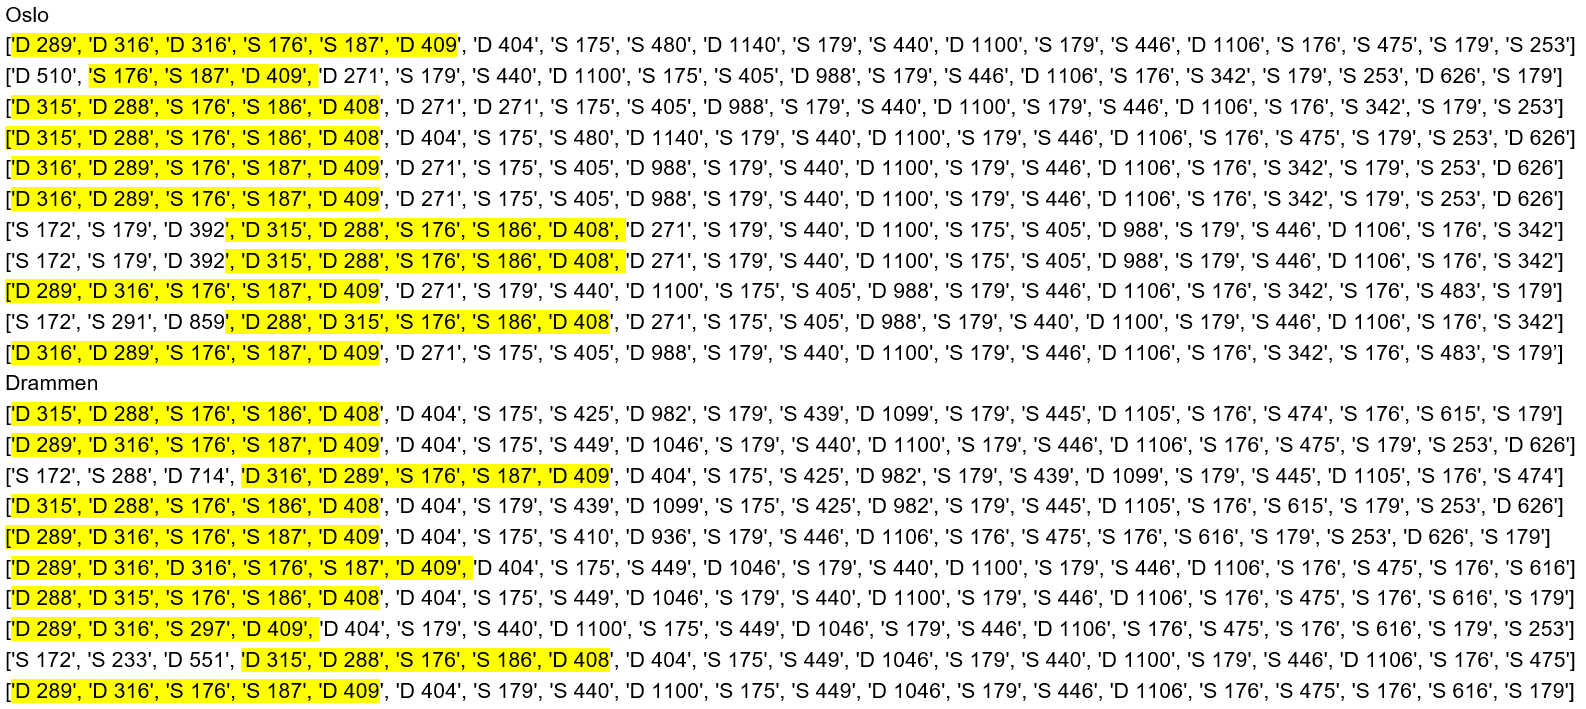
\includegraphics[width=\textwidth]{figures/Sequence_AC.png}
    \caption{Automated Cleaning extracted packet length sequences}
    \label{fig:ACseq}
\end{figure}

Both packet length sequences and the presence of two \gls{FQDN} are identified in all \textit{Automated cleaning} event captures. These observations forms the signature for this event. Two python functions were created: one for the detection of the \gls{DNS} responses for \textit{0550315.ingest.sentry.io} and \textit{s3.amazoneaws.com} and one to identify the packet sequences \textit{[315, 288, 176, 186, 408]} or \textit{[288, 315, 176, 186, 408]}. The pseudo code for \gls{DNS} detection is presented in Figure \ref{fig:pesudo_code_cleaning_event} and sequence detection in Figure \ref{fig:Pesudo_code_AC}.

\begin{figure}[H]
    \centering
    \begin{lstlisting}[numbers=left]
     function cleaning_event_detection(event_capture)
          if 'o550315.ingest.sentry.io' in event_capture
               dns1 == True
          elsif
               dns1 == False
          if 's3.amazonaws.com' in event_capture
               dns2 == True
          elsif
               dns2 == False
          if dns1 and dns2 == True      
               cleaning_confidence = + 10
          return cleaning_confidence
    \end{lstlisting}
    \caption{The algorithm for identifying \gls{DNS} responses for FQDNs \textit{0550315.ingest.sentry.io} and \textit{s3.amazoneaws.com}}
    \label{fig:pesudo_code_cleaning_event}
\end{figure}

\begin{figure}[H]
    \centering
    \begin{lstlisting}[numbers=left]
     function detect_application_start(packet_lengths_src)
          signature1 = [316, 289, 176, 187, 409]
          signature2 = [289, 316, 176, 187, 409]
          if signature1 in packet_lengths
               automated_cleaning_confidence = + 10
          elsif signature1 in packet_lengths
               automated_cleaning_confidence = + 10
    \end{lstlisting}
    \caption{The algorithm for identifying the \textit{Automated cleaning} packet length sequence}
    \label{fig:Pesudo_code_AC}
\end{figure}

To evaluate the detection algorithm it was used on all the different \textit{Automated cleaning} event files. The \gls{DNS} signature detection algorithm was able to identify the \gls{DNS} responses for \textit{0550315.ingest.sentry.io} and \textit{s3.amazoneaws.com} in all 20 event files. The sequence signature detection algorithm was able to identify the signature in 18 of 20 event files, resulting in a successful detection rate of 90\%. The two events that did not include this signature were Oslo event 2 and Drammen event 8, they had the sequences \textit{510, 176, 187, 409} and \textit{289, 316, 297, 409}. As mentioned in the sequence analysis the sequence detection will not be able to identify these.     

\section{Application Triggered Cleaning}

This section introduce specific configuration and decisions during the \textit{Application triggered cleaning} event triggering and analysis. The results from the analysis will be presented at the end of the section. 

\textit{Application triggered cleaning} is an event triggered manually by the Irobot Roomba's users through the Irobot home application's predefined or customized cleaning jobs. The event used a customized cleaning job defining the entire area of Oslo or Drammen smart map. This ensured that the cleaning area is constant for all the triggered events, creating the best foundation for comparison. These events can be triggered as many times as the user would like and is therefore the same during the entire capturing phase. 

Triggering date and time for all \textit{Application triggered cleaning} events are presented in Table \ref{tab:ATC_dateandtimeOslo} for Oslo and Table \ref{tab:ATC_dateandtimeDrammen} for Drammen. These events are triggered in a non-realistic manner due to time constrains, this is especially for the Drammen triggering where a new event was triggered every 30 minutes. In a realistic smart environment these triggerings would occur less and not in a structured manner. \textit{Application triggered cleaning} is triggered when the user needs additional cleaning outside of the scheduled one, preferably triggering this when leaving home. Identification of this event can therefore expose private information about user location. 

\begin{table}[H]
\centering
\caption{Application triggered cleaning triggering date and time overview for Oslo environment.}
\label{tab:ATC_dateandtimeOslo}
\begin{tabular}{|c|c|c|c|}
\hline
\textbf{Event} & \textbf{Date} & \textbf{Start time} & \textbf{End time} \\ \hline
1              & 28.02.2023         & 18:20               & 18:27             \\ \hline
2              & 28.02.2023         & 18:35               & 18:42             \\ \hline
3              & 01.03.2023         & 18:53               & 19:00             \\ \hline
4              & 09.03.2023         & 07:44               & 07:49             \\ \hline
5              & 09.03.2023         & 08:03               & 08:10             \\ \hline
6              & 09.03.2023         & 08:25               & 08:31             \\ \hline
7              & 09.03.2023         & 08:57               & 09:04             \\ \hline
8              & 09.03.2023         & 09:18               & 09:26             \\ \hline
9              & 12.03.2023         & 12:20               & 12:35             \\ \hline
10             & 12.03.2023         & 12:54               & 13:09             \\ \hline
\end{tabular}
\end{table}

\begin{table}[H]
\centering
\caption{Application triggered cleaning triggering date and time overview for Drammen environment.}
\label{tab:ATC_dateandtimeDrammen}
\begin{tabular}{|c|c|c|c|}
\hline
\textbf{Event} & \textbf{Date} & \textbf{Start time} & \textbf{End time} \\ \hline
1              & 25.02.2023         & 14:30               & 14:45             \\ \hline
2              & 25.02.2023         & 15:00               & 15:15             \\ \hline
3              & 25.02.2023         & 15:30               & 15:45             \\ \hline
4              & 25.02.2023         & 16:00               & 16:15             \\ \hline
5              & 25.02.2023         & 16:30               & 16:45             \\ \hline
6              & 25.02.2023         & 17:00               & 17:15             \\ \hline
7              & 25.02.2023         & 17:30               & 17:45             \\ \hline
8              & 25.02.2023         & 19:00               & 19:15             \\ \hline
9              & 25.02.2023         & 19:30               & 19:45             \\ \hline
10             & 25.02.2023         & 20:00               & 20:15             \\ \hline
\end{tabular}
\end{table}

Protocol distribution shows that there are two \gls{DNS} response packets in each of the event files, the rest of the traffic is \gls{TCP} where the majority are \gls{TLS} encrypted. \gls{TCP} packets without \gls{TLS} are either \gls{TCP} acknowledgement packets without payload or a part of a \gls{TCP} three-way-handshake or tare-down. When the event is triggered it is observed an increase in packets between the Irobot Roomba and the corresponding Irobot cloud server, this communication is at a consistent level until the cleaning is done. Then a \gls{DNS} response \gls{FQDN} \textit{0550315.ingest.sentry.io} is received and a new \gls{TCP} session to one of the responded \gls{IP} addresses is established. The entire corresponding \gls{TCP} session from Oslo environment event 5 is shown in Figure \ref{fig:ATC_DNS_ingest}, this is consistent for all \textit{Application triggered cleaning} events. After this session is finished a new \gls{DNS} response for \gls{FQDN} \textit{s3.amazoneaws.com} is received and a new \gls{TCP} session is established to one of the responded \gls{IP} addresses. 

\begin{figure}[H]
    \centering
    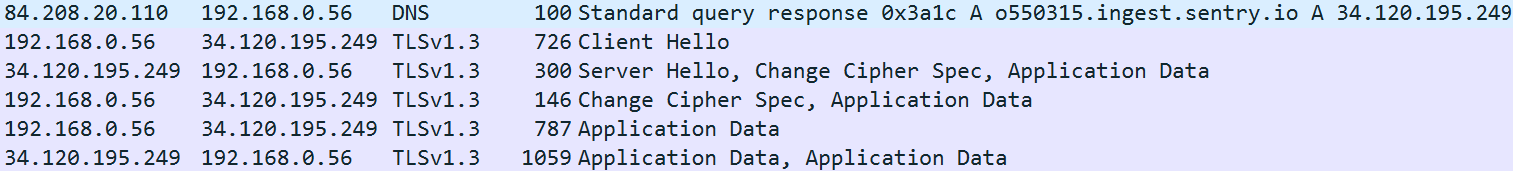
\includegraphics[width=\textwidth]{figures/irobot_ATC_DNSimgset.png}
    \caption{TCP session between Irobot Roomba and \textit{0550315.ingest.sentry.io}, initiated after application triggered cleaning is finished}
    \label{fig:ATC_DNS_ingest}
\end{figure}

Calculation of number of bytes and packets sent with associated average and standard deviation for all \textit{Application triggered cleaning} events are presented in Table \ref{tab:TCoverallOSL} and Table \ref{tab:TCoverallDRA}. Both number of packets and bytes sent are higher in Oslo despite shorter duration of cleaning, this could be environment specific due to floor, windows and furniture within each environment. More then 90\% of the packets are sent from the Irobot Roomba to \gls{FQDN} \textit{s3.amazoneaws.com}, as the majority of these packets are close to maximum packet size of 1,500 bytes they account for more then 95\% of the bytes transferred. This is most likely an upload of all the collected information form the cleaning. In Drammen environment both number of packets and bytes sent are increased for each consecutive event, based on similar duration and encrypted traffic it is not possible to determine why this occurred in Drammen. 

\begin{table}[H]
\centering
\caption{Application triggered cleaning, overall statistics Oslo}
\label{tab:TCoverallOSL}
\begin{tabular}{|c|c|c|}
\hline
\textbf{Event} & \textbf{Number of packets} & \textbf{Total number of bytes} \\ \hline
Event 1        & 2,667                   & 3,732,218                   \\ \hline
Event 2        & 2,686                   & 3,730,748                   \\ \hline
Event 3        & 2,656                   & 3,710,958                   \\ \hline
Event 4        & 3,065                   & 4,365,510                   \\ \hline
Event 5        & 2,880                   & 4,076,534                   \\ \hline
Event 6        & 2,633                   & 3,771,269                   \\ \hline
Event 7        & 2,661                   & 3,786,648                   \\ \hline
Event 8        & 2,647                   & 3,798,184                   \\ \hline
Event 9        & 2,729                   & 3,798,630                   \\ \hline
Event 10       & 2,639                   & 3,786,194                   \\ \hline
Average        & 2,726.3                 & 3,855,689.3                 \\ \hline
SD        & 139.57
       & 206,499.4               \\ \hline
\end{tabular}
\end{table}

\begin{table}[H]
\centering
\caption{Application triggered cleaning, overall statistics Drammen}
\label{tab:TCoverallDRA}
\begin{tabular}{|c|c|c|}
\hline
\textbf{Event} & \textbf{Number of packets} & \textbf{Number of bytes} \\ \hline
Event 1        & 708                    & 802,488                    \\ \hline
Event 2        & 724                    & 945,100                    \\ \hline
Event 3        & 740                    & 956,470                    \\ \hline
Event 4        & 809                    & 1,071,613                   \\ \hline
Event 5        & 824                    & 1,088,836                   \\ \hline
Event 6        & 869                    & 1,157,323                   \\ \hline
Event 7        & 855                    & 1,144,086                   \\ \hline
Event 8        & 929                    & 1,248,783                   \\ \hline
Event 9        & 988                    & 1,321,061                   \\ \hline
Event 10       & 983                    & 1,339,631                   \\ \hline
Average        & 842.9                  & 1,107,539.1                 \\ \hline
SD        & 101.85
       & 172,281.2               \\ \hline
\end{tabular}
\end{table}

The first 20 packet lengths of each of the \textit{Application triggered cleaning} events are extracted with the python script presented in Appendix \ref{app:Packetlengthex}. These sequences are manually analyzed to identify common packet length sequence to be used in event attribution. Packet lengths for all events are presented in Figure \ref{fig:ATCseq}, D and S indicate if the Irobot Roomba is destination or source of the packet. The yellow marked fields are the common sequences identified in the majority of event captures. Irobot cloud server is initiating the event with three packets with the length of \textit{[208, 288, 315]}, the last two packets can occur in mixed order, and all length can vary with one byte. Three packets are used to keep the complexity of the signature low. Identified sequence signature for \textit{Application triggered cleaning} is \textit{[208, 288, 315]} with the offset of 1 bytes for all packet sizes. Oslo event 9 is the only event capture wich does not include the identified signature, expected success rate of evaluation is therefore 95\%. 

\begin{figure}[H]
    \centering
    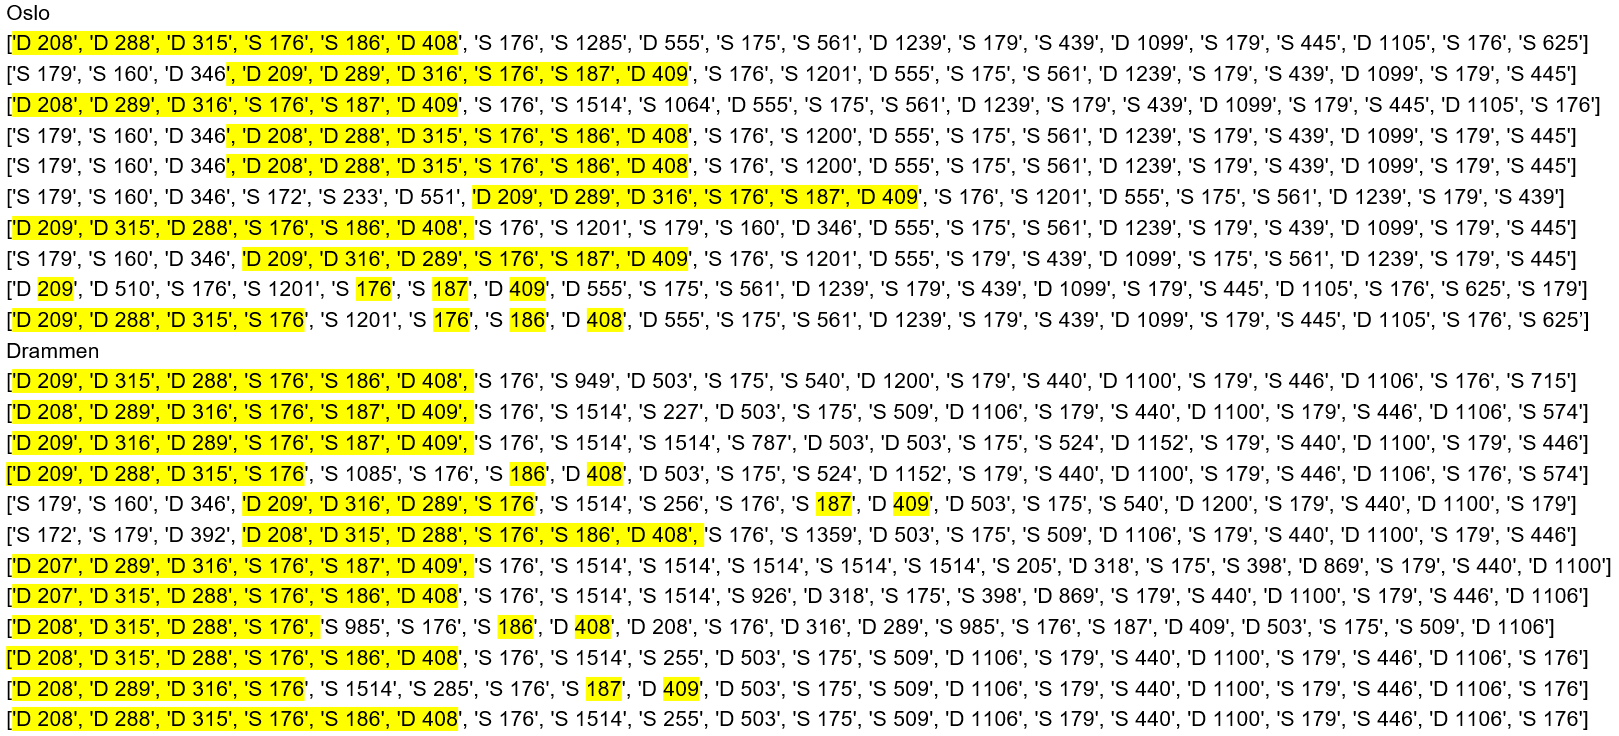
\includegraphics[width=\textwidth]{figures/Sequence_ATC.png}
    \caption{\textit{Application triggered} cleaning packet length sequence}
    \label{fig:ATCseq}
\end{figure}

To identify \textit{Application triggered cleaning} two detection algorithms are made, one identifying the \gls{DNS} responses \textit{0550315.ingest.sentry.io} and \textit{s3.amazoneaws.com} and one to identify the sequence signature specified above. Pseudo code for both algorithms are presented in Figure \ref{fig:pseudocodeATCDNS} and Figure \ref{fig:Sudo_code_ATC}.

\begin{figure}[H]
    \centering
    \begin{lstlisting}[numbers=left]
     function cleaning_event_detection(event_capture)
          if 'o550315.ingest.sentry.io' in event_capture
               dns1 == True
          elsif
               dns1 == False
          if 's3.amazonaws.com' in event_capture
               dns2 == True
          elsif
               dns2 == False
          if dns1 and dns2 == True      
               cleaning_confidence = + 10
          return cleaning_confidence
    \end{lstlisting}
    \caption{The algorithm for \gls{DNS} detection in Application triggered cleaning events}
    \label{fig:pseudocodeATCDNS}
\end{figure}

\begin{figure}[H]
    \centering
    \begin{lstlisting}[numbers=left]
     function detect_ATC(packet_lengths)
          signature1 = [209,289,316]
          signature2 = [209.316.289]
          if signature1 in packet_lengths
               ATC_confidence = + 10
          elsif signature1 in packet_lengths
              ATC_confidence = + 10
          return ATC_confidence
    \end{lstlisting}
    \caption{The algorithm for identifying the Application triggered cleaning packet sequence signature}
    \label{fig:Sudo_code_ATC}
\end{figure}

To evaluate the detection algorithms they are tested on all the capturing files for \textit{Application triggered cleaning}, trying to identify both signatures. The results of the identification are as expected,  \gls{DNS} detection had a success rate of 100\% and the sequence signature detection had a success rate of 95\%. The isolated event can therefore be identified with a high confidence, based on these results. 

\section{Scheduled Cleaning}
This section introduce specific configuration and decisions during \textit{Scheduled cleaning} event and analysis. The results from the analysis will be presented at the end of the section.

\textit{Scheduled cleaning} is triggered through configuration of customized cleaning jobs in the Irobot home application. A scheduled cleaning job was configured specifying the entire smart map as the cleaning area. Irobot restricts its users to not configure two scheduled cleanings with less then 3 hours space, cleaning jobs with less then 3 hours in between creates an error message. During this project only one scheduled clean was configured, but after the cleaning was finished the user entered the application changing the configured time. This enabled scheduled cleanings to be executed with less then 3 hours in between. It was observed that whenever a scheduled cleaning job was changed, the Irobot Roomba made a sound indicating that it got an update. The scheduled cleaning job is most likely sent to the vacuum cleaner at the time of configuration and then triggered locally. This way the Irobot Roomba is able to clean without Internet connection at the triggering time. 

Triggering dates and time for \textit{Scheduled cleaning} are presented in Table \ref{tab:SC_dateandtimeOslo} and \ref{tab:SC_dateandtimeDrammen}. These events are triggered in a non-realistic way due to time constrains, this is supported by Irobot's own restrictions mentioned above. Timings from \textit{Scheduled cleaning} can therefore not be used in the attribution of this specific event, however it would be a good indication if collected by an attack over a longer period of time. If a cleaning event is detected every Monday, Wednesday and Friday at 09:00 it is most likely due to scheduled cleaning, because a human triggered event would differ more in time. An observation during triggering was that the Irobot Roomba always started within 30 seconds before the scheduled time, this is also observed in the actual packet capture. In Figure \ref{fig:SC_start_time} event 2 in Oslo is shown, and there the traffic starts right before the scheduled timestamp. This is applicable for all events in the rage of 30-0 seconds before scheduled time. 

\begin{table}[H]
\centering
\caption{Scheduled cleaning triggering date and time overview for Oslo}
\label{tab:SC_dateandtimeOslo}
\begin{tabular}{|c|c|c|c|}
\hline
\textbf{Event} & \textbf{Date} & \textbf{Start time} & \textbf{End time} \\ \hline
1              & 10.03.2023         & 10:45               & 10:54             \\ \hline
2              & 10.03.2023         & 11:15               & 11:24             \\ \hline
3              & 10.03.2023         & 12:15               & 12:24             \\ \hline
4              & 10.03.2023         & 13:30               & 13:39             \\ \hline
5              & 10.03.2023         & 15:00               & 15:09             \\ \hline
6              & 10.03.2023         & 15:30               & 15:39             \\ \hline
7              & 10.03.2023         & 15:55               & 16:04             \\ \hline
8              & 10.03.2023         & 16:10               & 16:19             \\ \hline
9              & 11.03.2023         & 10:10               & 10:19             \\ \hline
10             & 11.03.2023         & 10:30               & 10:39             \\ \hline
\end{tabular}
\end{table}

\begin{table}[H]
\centering
\caption{Scheduled cleaning triggering date and time overview for Drammen}
\label{tab:SC_dateandtimeDrammen}
\begin{tabular}{|c|c|c|c|}
\hline
\textbf{Event} & \textbf{Date} & \textbf{Start time} & \textbf{End time} \\ \hline
1              & 25.02.2023         & 20:30               & 20:45             \\ \hline
2              & 25.02.2023         & 21:00               & 21:15             \\ \hline
3              & 26.02.2023         & 11:20               & 11:35             \\ \hline
4              & 26.02.2023         & 11:50               & 12:05             \\ \hline
5              & 26.02.2023         & 12:20               & 12:35             \\ \hline
6              & 26.02.2023         & 12:50               & 13:05             \\ \hline
7              & 26.02.2023         & 13:20               & 13:35             \\ \hline
8              & 26.02.2023         & 13:50               & 14:05             \\ \hline
9              & 26.02.2023         & 14:20               & 14:35             \\ \hline
10             & 26.02.2023         & 15:00               & 15:15             \\ \hline
\end{tabular}
\end{table}

\begin{figure}[H]
    \centering
    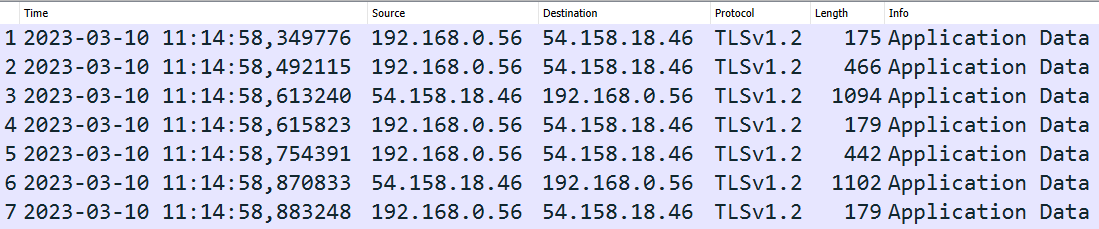
\includegraphics[width=\textwidth]{figures/SC_start_time.png}
    \caption{Start time for Scheduled cleaning in Oslo event 2, cleaning was scheduled 11:15}
    \label{fig:SC_start_time}
\end{figure}


Protocol distribution and overall traffic flow are similar as presented for \textit{Automated cleaning} and \textit{Application triggered cleaning}. The two same \gls{DNS} responses listed below are observed. 
\begin{itemize}
    \item 0550315.ingest.sentry.io
    \item s3.amazoneaws.com
\end{itemize}


Calculations of number of packets and bytes sent and \gls{SD} are presented in Table \ref{tab:scoverall} and Table \ref{tab:scoverallDRA}. Average and standard deviation in both Oslo and Drammen environment is small indicating small differences in the triggered events, this could be due to locally triggered events on the Irobot Roomba. 

\begin{table}[H]
\centering
\caption{Scheduled cleaning, overall statistics Oslo smart home}
\label{tab:scoverall}
\begin{tabular}{|c|c|c|}
\hline
\textbf{Event} & \textbf{Number of packets} & \textbf{Number of bytes} \\ \hline
Event 1        & 2,541                   & 3,669,941                   \\ \hline
Event 2        & 2,633                   & 3,678,959                   \\ \hline
Event 3        & 2,622                   & 3,660,004                   \\ \hline
Event 4        & 2,524                   & 3,629,262                   \\ \hline
Event 5        & 2,627                   & 3,658,515                   \\ \hline
Event 6        & 2,608                   & 3,729,110                   \\ \hline
Event 7        & 2,596                   & 3,645,238                   \\ \hline
Event 8        & 2,655                   & 3,685,536                   \\ \hline
Event 9        & 2,573                   & 3,713,211                   \\ \hline
Event 10       & 2,636                   & 3,768,883                   \\ \hline
Average        & 2,601.5                 & 3,683,865.9                 \\ \hline
SD       & 43.03       & 42,219.79               \\ \hline
\end{tabular}
\end{table}

\begin{table}[H]
\centering
\caption{Scheduled cleaning, overall statistics Drammen}
\label{tab:scoverallDRA}
\begin{tabular}{|c|c|c|}
\hline
\textbf{Event} & \textbf{Number of pkt} & \textbf{Number of bytes} \\ \hline
Event 1        & 996                    & 1,354,755                   \\ \hline
Event 2        & 1,052                   & 1,422,052                   \\ \hline
Event 3        & 1,150                   & 1,592,566                   \\ \hline
Event 4        & 1,317                   & 1,650,499                   \\ \hline
Event 5        & 1,166                   & 1,570,805                   \\ \hline
Event 6        & 1,179                   & 1,612,050                   \\ \hline
Event 7        & 1,160                   & 1,582,275                   \\ \hline
Event 8        & 1,177                   & 1,610,090                   \\ \hline
Event 9        & 1,205                   & 1,634,883                   \\ \hline
Event 10       & 1,170                   & 1,590,726                   \\ \hline
Average        & 1,157.2                 & 1,562,070.1                 \\ \hline
SD        & 85,66
       & 95,885,11               \\ \hline
\end{tabular}
\end{table}

The 20 first packet lengths were extracted with a python script presented in Appendix \ref{app:Packetlengthex}. The manual analysis of the packet lengths presented in Figure \ref{fig:Scseq}, resulted in two packet sequences of outbound traffic from the Irobot Roomba. The packet lengths varied more than previously and had a byte offset of 15 and 5 bytes depending on which signature sequence that was used. Both signature sequences are listed below with the associated byte offset. 

\begin{itemize}
    \item 176, 173, 179, 443, 177, byte offset 15 bytes 
    \item 176, 443, 179, 443, 177, byte offset 5 bytes
\end{itemize}

\begin{figure}[H]
    \centering
    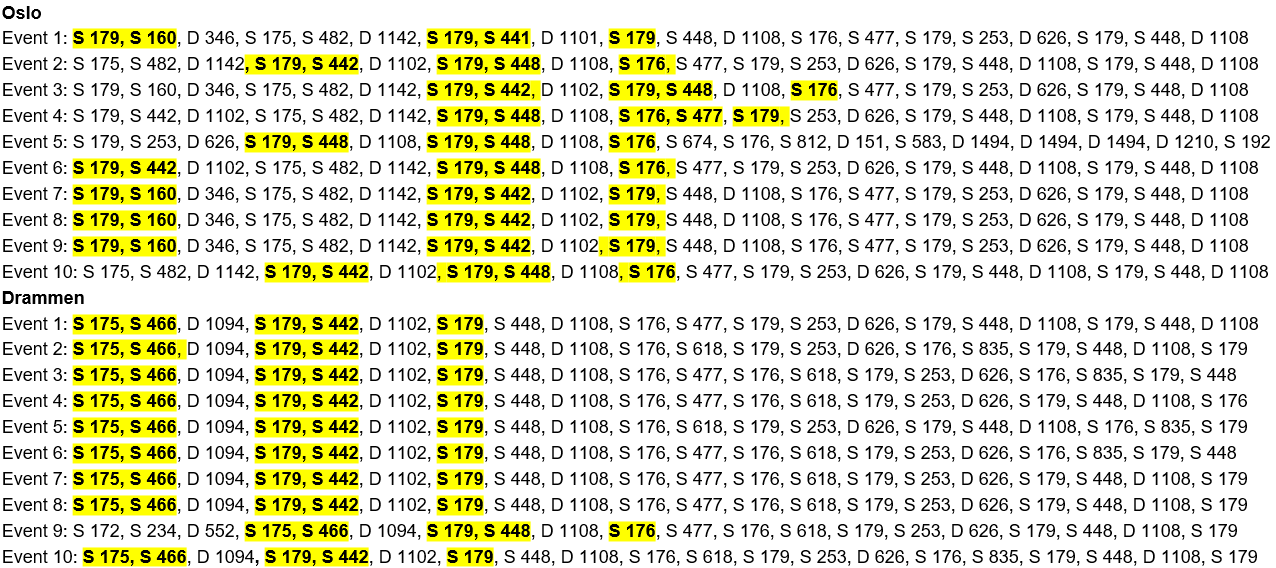
\includegraphics[width=\textwidth]{figures/Sequence_SC.png}
    \caption{\textit{Scheduled cleaning} packet length sequences}
    \label{fig:Scseq}
\end{figure}

As the \gls{DNS} signature is the same as for the two previous cleaning events analyzed, the same detection algorithm is used to evaluate this. Further, a new detection algorithm for the packet length sequence is presented in Figure \ref{fig:Sudo_code_SC_or_PC}. Both \gls{DNS} and sequence detection had a success rate of 100\% in all capturing files. Making this a good indication of the event if it is not detected in other events as well. 

\begin{figure}[H]
    \centering
    \begin{lstlisting}[numbers=left]
     function detect_application_start(packet_lengths_src)
          signature1 = [176,173,179,443,177]
          signature2 = = [176,443,179,443,177]
          if signature1 in packet_lengths
               SC_PTC_confidence = + 10
          elsif signature1 in packet_lengths
               SC_PTC_confidence = + 10
          return SC_PTC_confidence
    \end{lstlisting}
    \caption{Algorithm for scheduled cleaning packet sequence signature detection}
    \label{fig:Sudo_code_SC_or_PC}
\end{figure}


\section{Physical Triggered Cleaning}
This section introduce specific configuration and decisions during \textit{Physical triggered cleaning} event and analysis. The results from the analysis will be presented at the end of the section.

\textit{Physical triggered cleaning} events are only triggered by pressing the physical button on the Irobot Roomba. During triggering the user had to press the button twice to start the cleaning. Event triggering dates and time are presented in Table \ref{tab:PTC_dateandtimeOslo} and Table \ref{tab:PTC_dateandtimeDrammen}. The triggering in Oslo appears more realistic due to Drammen's strict triggering plan, these timestamps can therefore not be used to differentiate different cleaning events, but could have been a good indication if captured in a real-life smart environment. 

\begin{table}[H]
\centering
\caption{Physical triggered cleaning date and time overview for Oslo}
\label{tab:PTC_dateandtimeOslo}
\begin{tabular}{|c|c|c|c|}
\hline
\textbf{Event} & \textbf{Date} & \textbf{Start time} & \textbf{End time} \\ \hline
1              & 23.02.2023         & 18:08               & 18:24             \\ \hline
2              & 23.02.2023         & 18:36               & 19:05             \\ \hline
3              & 23.02.2023         & 19:14               & 19:34             \\ \hline
4              & 23.02.2023         & 20:13               & 20:35             \\ \hline
5              & 23.02.2023         & 20:44               & 21:06             \\ \hline
6              & 09.03.2023         & 09:43               & 10:02             \\ \hline
7              & 09.03.2023         & 10:30               & 10:50             \\ \hline
8              & 09.03.2023         & 12:32               & 12:50             \\ \hline
9              & 09.03.2023         & 13:16               & 14:05             \\ \hline
10             & 09.03.2023         & 17:44               & 18:05             \\ \hline
\end{tabular}
\end{table}

\begin{table}[H]
\centering
\caption{Physical triggered cleaning date and time overview for Drammen}
\label{tab:PTC_dateandtimeDrammen}
\begin{tabular}{|c|c|c|c|}
\hline
\textbf{Event} & \textbf{Date} & \textbf{Start time} & \textbf{End time} \\ \hline
1              & 25.02.2023         & 22:00               & 22:12             \\ \hline
2              & 25.02.2023         & 22:30               & 22:45             \\ \hline
3              & 25.02.2023         & 23:00               & 23:15             \\ \hline
4              & 25.02.2023         & 23:20               & 23:35             \\ \hline
5              & 25.02.2023         & 23:40               & 23:55             \\ \hline
6              & 26.02.2023         & 00:00               & 00:15             \\ \hline
7              & 26.02.2023         & 00:20               & 00:35             \\ \hline
8              & 26.02.2023         & 00:40               & 00:55             \\ \hline
9              & 26.02.2023         & 01:06               & 01:20             \\ \hline
10             & 26.02.2023         & 01:31               & 01:45             \\ \hline
\end{tabular}
\end{table}

Protocol distribution and traffic flow are similar as in the other three cleanings events presented above. The two same \gls{DNS} responses are identified as well as their corresponding \gls{TCP} sessions. Standard deviation for both environments are small, indicating that the events are similar and supporting that the hypothesis on 20 events are sufficient. 

\begin{table}[H]
\centering
\caption{Physical triggered cleaning, overall statistics Oslo}
\label{tab:PCoverallOSL}
\begin{tabular}{|c|c|c|}
\hline
\textbf{Event} & \textbf{Number of packets} & \textbf{Number of bytes} \\ \hline
Event 1        & 2,791                   & 3,965,147                   \\ \hline
Event 2        & 3,180                   & 4,357,126                   \\ \hline
Event 3        & 2,926                   & 4,033,946                   \\ \hline
Event 4        & 2,872                   & 4,112,516                   \\ \hline
Event 5        & 2,944                   & 4,209,443                   \\ \hline
Event 6        & 2,984                   & 4,122,412                   \\ \hline
Event 7        & 2,925                   & 4,160,462                   \\ \hline
Event 8        & 2,869                   & 4,100,166                   \\ \hline
Event 9        & 2,918                   & 4,227,626                   \\ \hline
Event 10       & 2,768                   & 3,957,559                   \\ \hline
Average        & 2,917.7                 & 4,124,640.3                 \\ \hline
SD        & 113.98
       & 122,683.4               \\ \hline
\end{tabular}
\end{table}

\begin{table}[H]
\centering
\caption{Physical triggered cleaning, overall statistics Drammen}
\label{tab:PCoverallDRA}
\begin{tabular}{|c|c|c|}
\hline
\textbf{Event} & \textbf{Number of packets} & \textbf{NUmber of bytes} \\ \hline
Event 1        & 1,078                   & 1,481,677                   \\ \hline
Event 2        & 1,087                   & 1,484,930                   \\ \hline
Event 3        & 1,125                   & 1,520,872                   \\ \hline
Event 4        & 1,088                   & 1,517,429                   \\ \hline
Event 5        & 1,150                   & 1,555,605                   \\ \hline
Event 6        & 1,086                   & 1,507,084                   \\ \hline
Event 7        & 1,092                   & 1,501,894                   \\ \hline
Event 8        & 1,115                   & 1,510,971                   \\ \hline
Event 9        & 1,098                   & 1,485,863                   \\ \hline
Event 10       & 1,100                   & 1,492,331                   \\ \hline
Average        & 1,101.9                 & 1,505,865.6                 \\ \hline
SD        &22.05
       & 22,318.19               \\ \hline
\end{tabular}
\end{table}

The first 20 packet lengths are extracted with the same python script as for the other events, presented in Appendix \ref{app:Packetlengthex}. Analysis resulted in the identification of the same packet sequence as for \textit{Scheduled cleaning} event, this could be because these two events are both triggered on the Irobot Roomba locally and not initiated from the Irobot cloud server. If this is the reason, the identified sequence could be present in all cleaning events. The extracted sequences are presented in Figure \ref{fig:PCseq}, yellow marked are the identified sequence and D and S represents if the Irobot Roomba is destination or source of the packet. 

\begin{figure}[H]
    \centering
    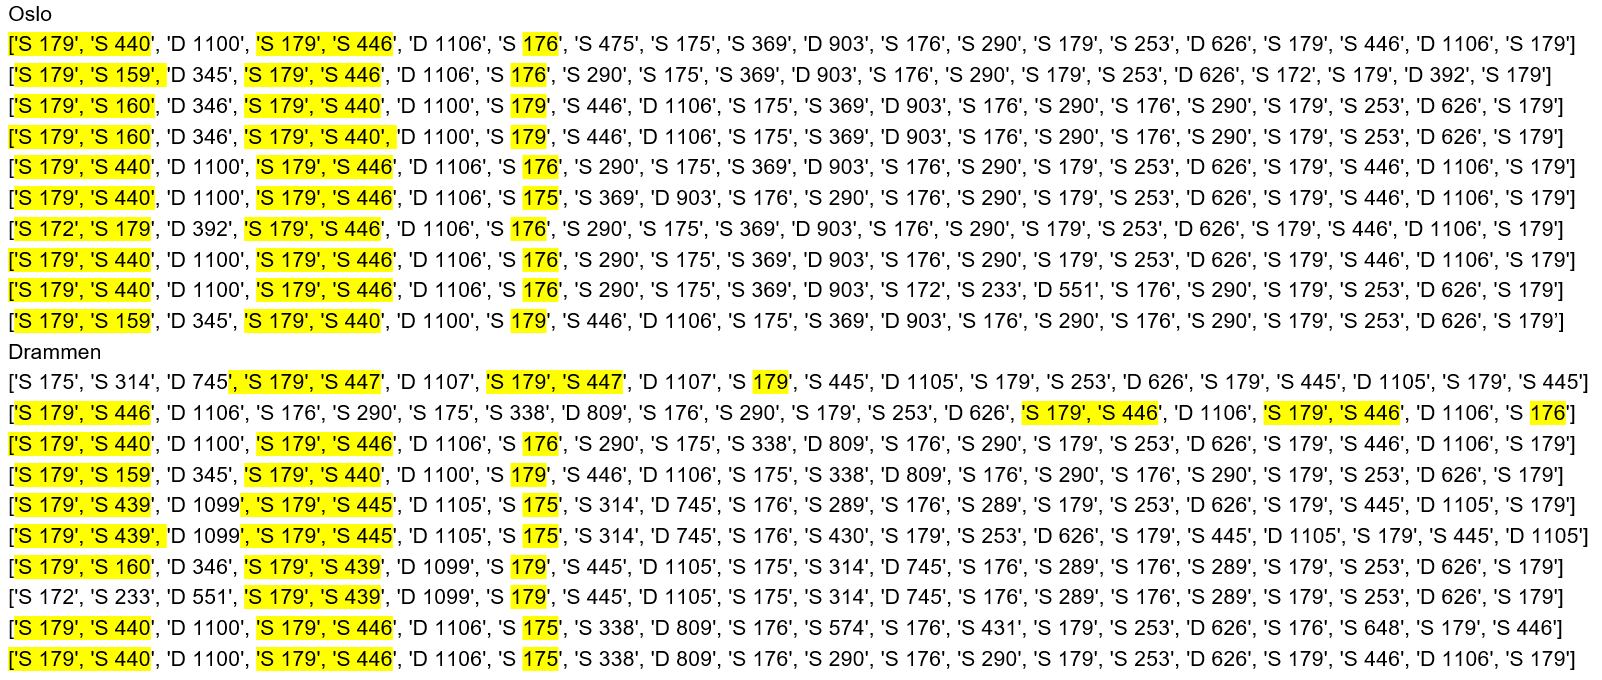
\includegraphics[width=\textwidth]{figures/Sequence_PC.png}
    \caption{Physical triggered cleaning packet length sequences}
    \label{fig:PCseq}
\end{figure}

The identified signatures are identical as for \textit{Scheduled cleaning}, the two same signature detection algorithms were used to evaluate the findings. Both algorithms had a 100\% success rate for identifying \textit{Physical triggered cleaning}, this means that neither of the events can be distinguished with these signatures. This attribution could been done by using timestamps, but the events in this research have too unrealistic triggering. 

\section{Application Start}
This section introduce specific configuration and decisions during \textit{Application start} event and analysis. The results from the analysis will be presented at the end of the section.

\textit{Application start} events are triggered by the user opening the Irobot application. Triggering dates and times are presented in Table \ref{tab:AS_dateandtimeOslo} and Table \ref{tab:AS_dateandtimeDrammen}. No specific action was defined during the event, so several different actions was executed such as, changing scheduled cleaning time, watch the dashboard and display configuration. Only the initial event traffic will therefore be included in the application open event. 

\begin{table}[H]
\centering
\caption{Application start event date and time overview for Oslo}
\label{tab:AS_dateandtimeOslo}
\begin{tabular}{|c|c|c|c|}
\hline
\textbf{Event} & \textbf{Date} & \textbf{Start time} & \textbf{End time} \\ \hline
1              & 10.03.2023         & 10:26               & 10:27             \\ \hline
2              & 10.03.2023         & 11:06               & 11:07             \\ \hline
3              & 10.03.2023         & 11:56               & 11:57             \\ \hline
4              & 10.03.2023         & 13:22               & 13:23             \\ \hline
5              & 10.03.2023         & 14:58               & 14:59             \\ \hline
6              & 10.03.2023         & 15:27               & 15:28             \\ \hline
7              & 10.03.2023         & 15:51               & 15:52             \\ \hline
8              & 10.03.2023         & 16:07               & 16:08             \\ \hline
9              & 11.03.2023         & 10:06               & 10:07             \\ \hline
10             & 11.03.2023         & 10:22               & 10:23             \\ \hline
\end{tabular}
\end{table}

\begin{table}[H]
\centering
\caption{Application start event date and time overview for Drammen}
\label{tab:AS_dateandtimeDrammen}
\begin{tabular}{|c|c|c|c|}
\hline
\textbf{Event} & \textbf{Date} & \textbf{Start time} & \textbf{End time} \\ \hline
1              & 25.02.2023         & 20:50               & 20:52             \\ \hline
2              & 25.02.2023         & 21:20               & 21:21             \\ \hline
3              & 25.02.2023         & 22:20               & 22:22             \\ \hline
4              & 25.02.2023         & 22:50               & 22:52             \\ \hline
5              & 26.02.2023         & 11:10               & 11:11             \\ \hline
6              & 26.02.2023         & 11:40               & 11:41             \\ \hline
7              & 26.02.2023         & 12:10               & 12:11             \\ \hline
8              & 26.02.2023         & 12:40               & 12:41             \\ \hline
9              & 26.02.2023         & 13:10               & 13:11             \\ \hline
10             & 26.02.2023         & 13:40               & 13:41             \\ \hline
\end{tabular}
\end{table}

The protocol distribution analysis identified only \gls{TCP} packets, no \gls{DNS} packets is sent during the event, indication that the requested information pulled from the Irobot Roomba when the application is started is initiated from \textit{a2uowfjvhio0fa.iot.us-east-1.amazonaws.com}. If the smart phone had been located in the same smart environment, it could be possible to identify a \gls{DNS} request to this service. No standard action was performed in the application during this event, the standard deviation from the calculations presented in Table \ref{tab:ASoverallOslo} and Table \ref{tab:ASoverallDRA} is therefore large, and only the initiating traffic is relevant to this analysis. During event 5-10 in Drammen, the user performed a scheduled clean configuration resulting in a high number of bytes sent compared to some of the other events.  

\begin{table}[H]
\centering
\caption{Application start event overall statistics Oslo}
\label{tab:ASoverallOslo}
\begin{tabular}{|l|l|l|}
\hline
\textbf{Event} & \textbf{Number of packets} & \textbf{Number of bytes} \\ \hline
Event 1        & 11                     & 5,202                      \\ \hline
Event 2        & 22                     & 8,698                      \\ \hline
Event 3        & 20                     & 8,644                      \\ \hline
Event 4        & 17                     & 7,135                      \\ \hline
Event 5        & 20                     & 8,580                      \\ \hline
Event 6        & 20                     & 8,608                      \\ \hline
Event 7        & 20                     & 9,213                      \\ \hline
Event 8        & 23                     & 9,527                      \\ \hline
Event 9        & 20                     & 8,730                      \\ \hline
Event 10       & 19                     & 8,877                      \\ \hline
Average        & 19.2                   & 8,321.4                    \\ \hline
SD        & 3.29
       & 1,258.62               \\ \hline
\end{tabular}
\end{table}

\begin{table}[H]
\centering
\caption{Application start, overall statistics Drammen}
\label{tab:ASoverallDRA}
\begin{tabular}{|l|l|l|}
\hline
\textbf{Event} & \textbf{Packet number} & \textbf{Total bytes sent} \\ \hline
Event 1        & 30                     & 20,875                     \\ \hline
Event 2        & 26                     & 19,568                     \\ \hline
Event 3        & 8                      & 2,655                      \\ \hline
Event 4        & 8                      & 2,659                      \\ \hline
Event 5        & 26                     & 19,561                     \\ \hline
Event 6        & 34                     & 21,897                     \\ \hline
Event 7        & 29                     & 20,222                     \\ \hline
Event 8        & 25                     & 19,468                     \\ \hline
Event 9        & 33                     & 21,744                     \\ \hline
Event 10       & 26                     & 19,570                     \\ \hline
Average        & 24,5                   & 16,821.9                   \\ \hline
SD       & 9.22
       & 7.519.30               \\ \hline
\end{tabular}
\end{table}

The first 20 packet lengths were extracted with the python script presented in Appendix \ref{app:Packetlengthex}, and the result is presented in Figure \ref{fig:ASseq}. The yellow marked fields are a part of the identified packet length sequence. The identified sequences are \textit{[209, 288, 315]} and \textit{[209, 315, 288]}, where both sequences have an offset of 1 byte. This is the same packet sequence signature as identified in \textit{Application triggered cleaning}, and is therefore used to identify \textit{Application start}. These sequences are therefore generated whenever the Irobot home application is started. To differentiate these two events the \gls{DNS} signature found in all cleaning events have to be identified.  

\begin{figure}[H]
    \centering
    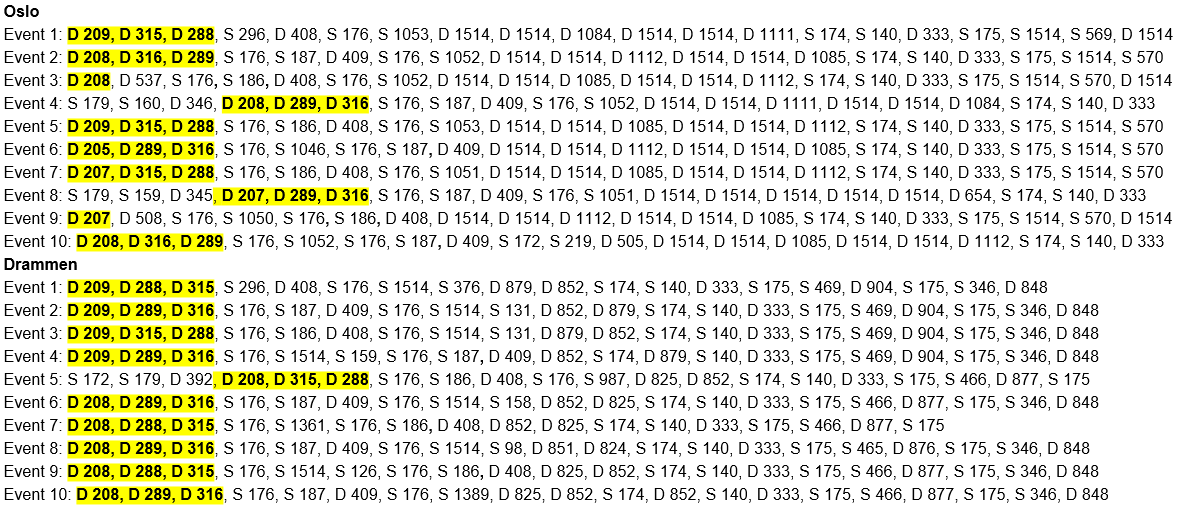
\includegraphics[width=\textwidth]{figures/Sequence_AS.png}
    \caption{Application start packet length sequences}
    \label{fig:ASseq}
\end{figure}

Evaluation of \textit{Application start} detection is determined with the same packet length sequence detection algorithm presented in Figure \ref{fig:Sudo_code_ATC}. This detection had a success rate of 90\% detection of the event, and it is therefore possible to determine that the application is started with high confidence.

\section{Bin Remove}
This section introduce specific configuration and decisions during \textit{Bin remove} event and analysis. The results from the analysis will be presented at the end of the section.

\textit{Bin remove} is triggered when the physical bin eject button is pressed on the Irobot Roomba i7 and the bin is then released. It is injected by pushing the bin back into place. Triggering dates and times are presented in Table \ref{tab:BR_dateandtimeOslo} and \ref{tab:BR_dateandtimeDrammen}, intervals between the triggering is small, but in analysis it was possible to differentiate when the different traffic occurred. During event triggering the response from the Irobot Roomba was variable, sometimes it flashed and sometimes it did not respond at all. The flashing is due to the Irobot Roomba loosing connection to the charger and not ejection of the bin. The amount of packets and bytes are also variable most likely due to the inconsistent in the event triggering process, resulting in a high standard deviation. These calculations are presented in Table \ref{tab:BRoverallOslo} and Table \ref{tab:BRoverallDRA}. 

\begin{table}[H]
\centering
\caption{Bin remove date and time overview for Oslo}
\label{tab:BR_dateandtimeOslo}
\begin{tabular}{|c|c|c|c|}
\hline
\textbf{Event} & \textbf{Date} & \textbf{Start time} & \textbf{End time} \\ \hline
1              & 11.03.2023    & 17:30               & 17:31             \\ \hline
2              & 11.03.2023    & 17:35               & 17:36             \\ \hline
3              & 11.03.2023    & 17:40               & 17:41             \\ \hline
4              & 11.03.2023    & 17:44               & 17:45             \\ \hline
5              & 11.03.2023    & 17:47               & 17:48             \\ \hline
6              & 11.03.2023    & 17:49               & 17:50             \\ \hline
7              & 11.03.2023    & 17:51               & 17:52             \\ \hline
8              & 11.03.2023    & 17:53               & 17:54             \\ \hline
9              & 11.03.2023    & 17:55               & 17:56             \\ \hline
10             & 11.03.2023    & 18:01               & 18:02             \\ \hline
\end{tabular}
\end{table}

\begin{table}[H]
\centering
\caption{Bin remove date and time overview for Drammen}
\label{tab:BR_dateandtimeDrammen}
\begin{tabular}{|c|c|c|c|}
\hline
\textbf{Event} & \textbf{Date} & \textbf{Start time} & \textbf{End time} \\ \hline
1              & 26.02         & 15:22               & 15:23             \\ \hline
2              & 26.02         & 15:30               & 15:31             \\ \hline
3              & 26.02         & 15:35               & 15:36             \\ \hline
4              & 27.02         & 15:05               & 15:06             \\ \hline
5              & 27.02         & 15:10               & 15:11             \\ \hline
6              & 27.02         & 15:15               & 15:16             \\ \hline
7              & 27.02         & 15:20               & 15:21             \\ \hline
8              & 27.02         & 15:25               & 15:26             \\ \hline
9              & 27.02         & 15:30               & 15:31             \\ \hline
10             & 27.02         & 15:35               & 15:36             \\ \hline
\end{tabular}
\end{table}

\begin{table}[H]
\centering
\caption{Bin remove, overall statistics Oslo}
\label{tab:BRoverallOslo}
\begin{tabular}{|l|l|l|}
\hline
\textbf{Event} & \textbf{Packet number} & \textbf{Total bytes sent} \\ \hline
Event 1        & 6                      & 2,512                      \\ \hline
Event 2        & 15                     & 5,765                      \\ \hline
Event 3        & 12                     & 4,366                      \\ \hline
Event 4        & 15                     & 7,869                      \\ \hline
Event 5        & 12                     & 5,022                      \\ \hline
Event 6        & 17                     & 8,426                      \\ \hline
Event 7        & 18                     & 8,492                      \\ \hline
Event 8        & 12                     & 5,022                      \\ \hline
Event 9        & 11                     & 4,956                      \\ \hline
Event 10       & 12                     & 5,022                      \\ \hline
Average        & 13                     & 5,745.2                    \\ \hline
SD        & 3.43
       & 1,937.64               \\ \hline
\end{tabular}
\end{table}


\begin{table}[H]
\centering
\caption{Bin remove, overall statistics Drammen }
\label{tab:BRoverallDRA}
\begin{tabular}{|l|l|l|}
\hline
\textbf{Event} & \textbf{Packet number} & \textbf{Total bytes sent} \\ \hline
Event 1        & 23                     & 8,610                      \\ \hline
Event 2        & 24                     & 10,149                     \\ \hline
Event 3        & 9                      & 4,407                      \\ \hline
Event 4        & 12                     & 5,022                      \\ \hline
Event 5        & 8                      & 4,333                      \\ \hline
Event 6        & 9                      & 4,399                      \\ \hline
Event 7        & 17                     & 6,595                      \\ \hline
Event 8        & 9                      & 4,399                      \\ \hline
Event 9        & 15                     & 7,869                      \\ \hline
Event 10       & 12                     & 5,022                      \\ \hline
Average        & 13,8                   & 6,080.5                    \\ \hline
SD        & 5.87
       & 2,112.52               \\ \hline
\end{tabular}
\end{table}

Packet length sequences were extracted with the python script in Appendix \ref{app:Packetlengthex}, and the results are presented in Figure \ref{fig:BRseq}. The identified sequences are marked in yellow, packets with the length of \textit{410 or 411} bytes were observed, these lengths are not observed in other events and is defined as the sequence signature for \textit{Bin remove}. The detection algorithm created is presented in pseudo code in Figure \ref{fig:Sudo_code_BinRemove} and is used to identify the signature in all event capture files. The evaluation result of testing is 100\% success rate of signature detection.   

\begin{figure}[H]
    \centering
    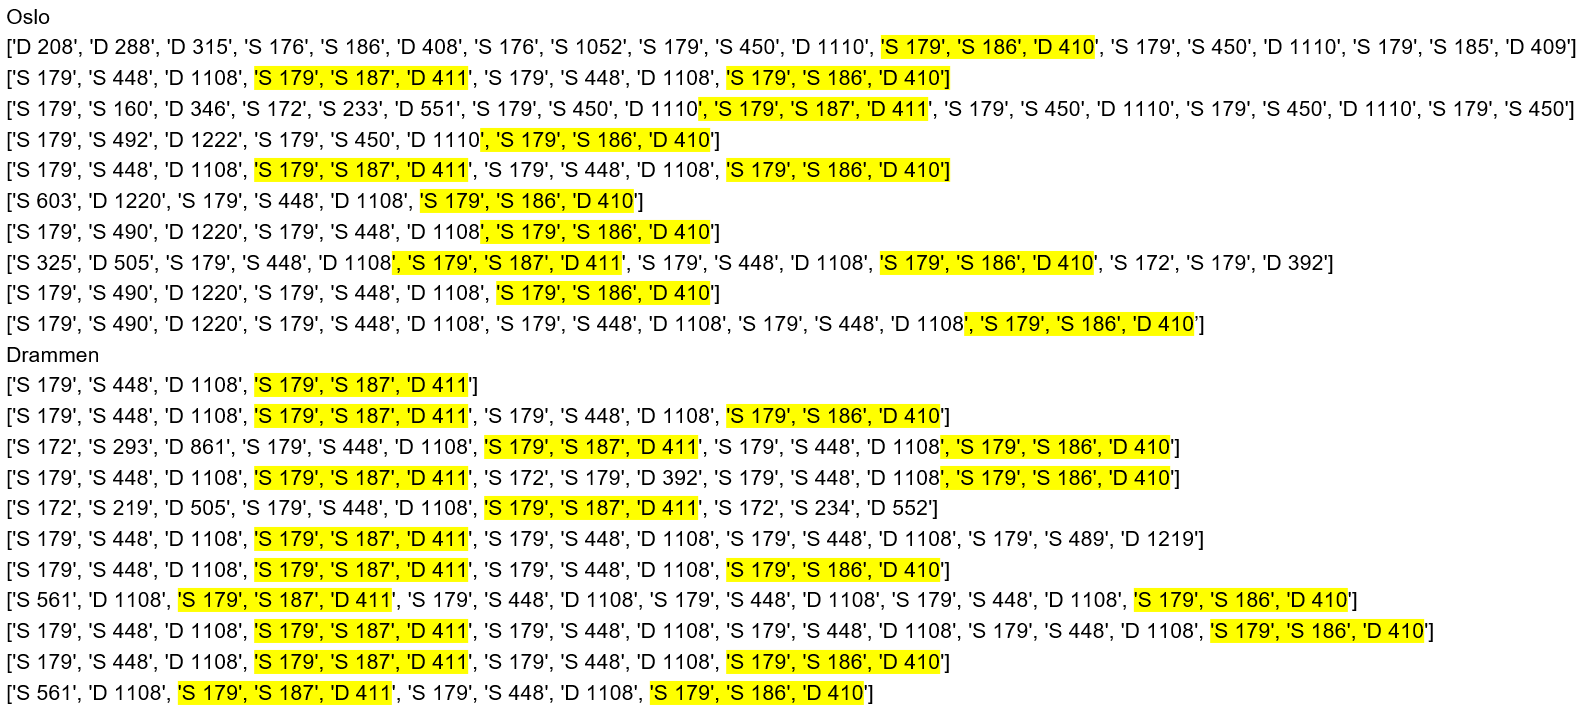
\includegraphics[width=\textwidth]{figures/Sequence_BR.png}
    \caption{Bin remove packet length sequences}
    \label{fig:BRseq}
\end{figure}

\begin{figure}[H]
    \centering
    \begin{lstlisting}[numbers=left]
     function bin_remove(br_confidence)
          if packet.length == 410 or 411 in capture.file
              br_confident = + 10
          return br_confident
    \end{lstlisting}
    \caption{Pseudo code for detection algorithm for \textit{Physical triggered cleaning} packet length sequence}
    \label{fig:Sudo_code_BinRemove}
\end{figure}

\section{Signature Comparison}
This section will present the comparison of the different signatures used for event attribution in the sections above. First an evaluation test where all signatures are tested on all events to identify if the signatures are unique. This is followed by an analysis of the evaluation results.

 \textit{Remove bin} signature seems to be detected in all events except \textit{Application start}, this signature is therefore removed from further analysis. 

All the different cleaning events, \textit{Automated cleaning, Scheduled cleaning, Application triggered cleaning} and \textit{Physical triggered cleaning} had the same \gls{DNS} responses present in the packet capturing. First a \gls{DNS} response for \gls{FQDN} \textit{0550315.ingest.sentry.io}, followed by a response for\textit{s3.amasoneaws.com}. These \gls{DNS} packets can therefore not be used as signature for any of the specific cleaning events, but can increase confidence in a cleaning detection. However there are several similarities between the identified sequences and this will be discussed further.

Signature sequence can not differentiate between \textit{Scheduled cleaning} or \textit{Physical triggered cleaning}. However the traffic sequence on all the scheduled cleaning events is started within a minute before the scheduled cleaning's configured triggering time. It is safe to assume that scheduled cleaning is configured every whole hour or half hour. A normal user would not configure a cleaning at 15:17, but more likely at 15:00. If an attacker is monitoring a smart environment during a longer time period, the two different cleanings can be separated based on reoccurring identification. A identified cleaning every Monday at 07:59 is most likely a scheduled cleaning, since humans are unable to provide the same level of consistency as \gls{IoT} devices.

We can assume that the sequence used to identify \textit{Application triggered cleaning} and \textit{Application start} is due to the fact that the application is started, and not the actual triggering of the cleaning event. It is still possible to differentiate between these two events with the use of cleaning \gls{DNS} signature. As all other cleaning events, it includes a \gls{DNS} response for \gls{FQDN} \textit{0550315.ingest.sentry.io} and then \textit{s3.amazoneaws.com}. If the \textit{Application start} sequences and the cleaning \gls{DNS} responses are detected, an application triggered cleaning is most likely executed. An element of uncertainty occurs if the user opens the application before or during another cleaning event, then this could create a false positive. 

The only difference between \textit{Automated cleaning} and \textit{Application triggered cleaning} is the first package in the sequence of \textit{Application start}. This packet has the length of 209 or 208 bytes and occurs every time the application is started. The identification of this is therefore a good attribute to differentiate for these events.

\section{Wireless and Wired Traffic Capture Comparison}
This section will compare the corresponding \gls{LAN} and \gls{WLAN} captures, and determine if the same method and identification can be applicable to identify events only based on wireless traffic as well. 

\gls{WLAN} and \gls{LAN} traffic were captured for all triggered events, but due to the thesis' time constrains only identification of signatures and detection algorithms on \gls{LAN} captures was conducted. The simulated \gls{WAN} traffic had more available attributes, due to the \gls{Wi-Fi}'s encryption. In  \cite{pingpong_trimananda2020packet} they have already proposed a method to identify actions based on packet lengths. This research therefore focused on the \gls{WAN} traffic, to be able to include \gls{DNS} as an identifier. To evaluate if the same method and algorithms are applicable to \gls{WLAN} traffic a comparison of two corresponding captures was done. Through analysis we identified that the added \gls{Wi-Fi} header was 79 bytes and the base filter of 97 bytes in \gls{LAN} captures was therefore converted to 176 bytes in \gls{WLAN}. When this filter was applied, the same packet sequences as in the simulated \gls{WAN} traffic were observed. These findings are presented in Figure \ref{fig:WLANLANHeader}. With the basefilter applied, it was observed that the \gls{WLAN} capture included less packets than the corresponding \gls{LAN} capture. This could be the result of retransmission, dual \gls{Wi-Fi} channels, signal disruption or packet collision on the \gls{NIC} in monitoring mode. When the \gls{NIC} was configured in monitoring mode, it collected all \gls{Wi-Fi} traffic in the area. This includes traffic from other \gls{SSID}s within wireless coverage. The original \gls{ISP} modem was also broadcasting it's \gls{SSID}s, causing high Signal to Noise Ratio (SnR) for more than one \gls{SSID}. Without control traffic between the \gls{AP} and the \gls{NIC} it could potentially lose traffic. Regardless of the packet loss it is still possible to identify similar patterns in \gls{WLAN} traffic as in \gls{LAN} traffic. 

\begin{figure}[H]
    \centering
    \begin{subfigure}[b]{0.9\textwidth}
        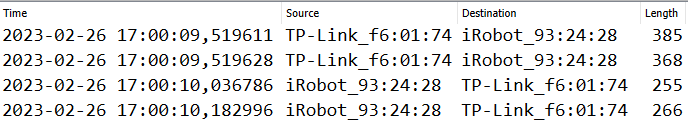
\includegraphics[width=\textwidth]{figures/WLANLANComparison.png}
        \caption{\gls{WLAN}}
    \end{subfigure}
    \quad
    \begin{subfigure}[b]{0.9\textwidth}
        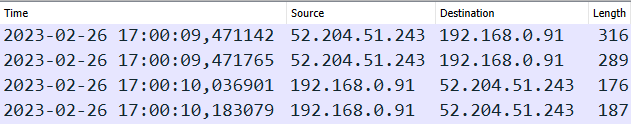
\includegraphics[width=\textwidth]{figures/LANWLANcomparison.png}
        \caption{\gls{LAN}}
    \end{subfigure}
    
    \caption{\gls{WLAN} and \gls{LAN} comparison}
    \label{fig:WLANLANHeader}
\end{figure}

\gls{WLAN} captures need more analysis before they can be implemented in the detection algorithm. An advantage of \gls{WLAN} traffic is the availability of \gls{MAC} addresses, an attacker can therefore easily identify the robot vacuum cleaner and filter traffic based on this information. Compared to \gls{LAN} where an attacker will have to eavesdrop for up to 24 hours before the Irobot traffic can be identified. 

Number of packets or bytes transmitted could also be used as an attribute to identify that there has been triggered a cleaning within the smart environment. This detection will be applicable for both \gls{LAN} and \gls{WLAN} eavesdropping.  